%!TEX root = ./Thesis.tex
\chapter{Discrete Differential Geometry - Software Packages}

\section{Introduction}

\begin{figure}[h]
	\centering
	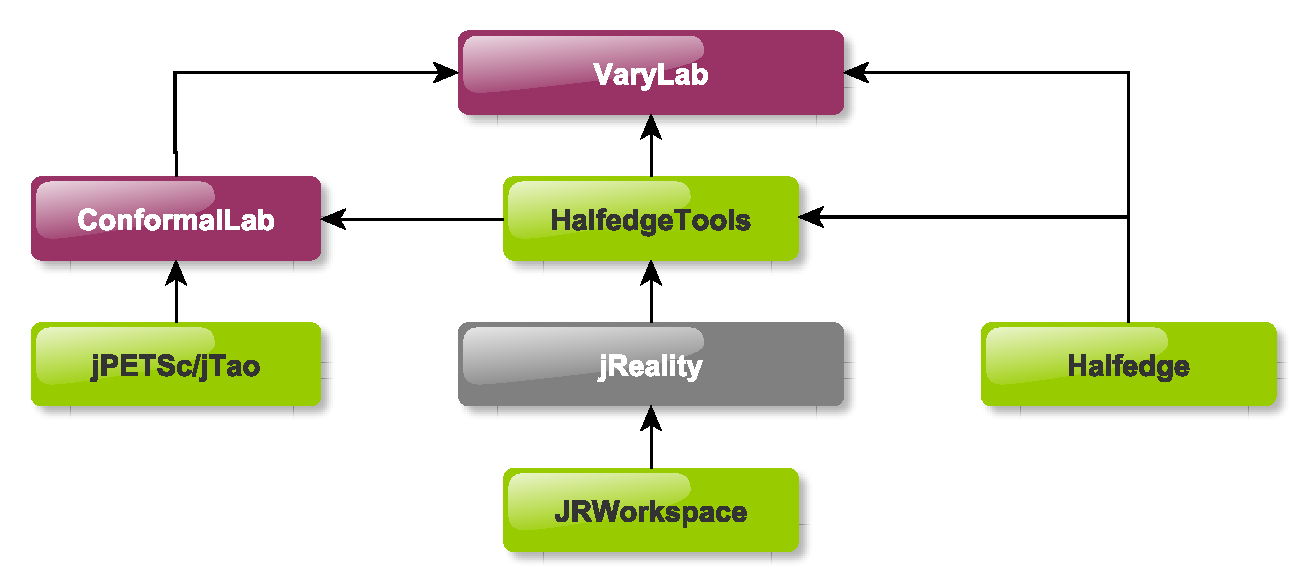
\includegraphics[width=\linewidth]{figures/software_architecture}
	\caption[Software package dependencies]{
		Software architecture and dependencies of the DDG Framework. 
		{\sc Jtem} library packages (green), mathematical software packages (red).
	}
	\label{fig:software_architecture}
\end{figure}

In the field of Discrete Differential Geometry (DDG) there is a special need for experiments
conducted with the help of computer software. Especially if the methods of DDG are applied
to problems in computer graphics, geometry processing, or architecture, algorithms have 
to be implemented and convincing examples have to be presented. Additionally a suitable 
visualization of the results has to be included in a state-of-the-art publication.

There is a growing knowledge of software development in the mathematical community. This 
is due to the curricula of universities which started to include programming courses for 
undergraduate students with a visualization emphasis, e.g., \cite{VisMathHomepage, 
CaltechVisMath}. It enables students to extend their abilities of creating visualizations and 
mathematical software, where former generations of students solely used the visualization 
abilities of standard computer algebra packages like Mathematica or MatLab.

The audience of this chapter is two-fold. On the one hand it is students creating their 
visualizations of surfaces and develop algorithms. On the other hand it is researchers in the
field of discrete differential geometry who need a stable data structure and programming
infrastructure to get the job done.

This Chapter is the description and getting-started manual of a set of software packages
(Berlin DDG Framework) written in the programming language {\sc Java}. They are 
specifically designed for the creation of
custom interactive software for experiments with algorithms and geometries treated 
within DDG. It is currently beeing used for teaching a mathematical visualization course at 
TU-Berlin \cite{VisMathHomepage} and for research projects within the geometry group.

Section~\ref{sec:related_work} gives an overview of existing software packages that have a focus 
similar to the DDG Framework. Section~\ref{sec:jrworkspace} introduces the {\sc JRworkspace} library of the 
{\sc Jtem} project~\cite{JtemWebsite}. It is the foundation of any application created with 
the DDG Framework. It is also the user interface basis of {\sc Jreality}, a mathematical 
visualization library that uses {\sc JRworkspace} as plug-in and user interface 
tool~\cite{JrealityWebsite}. Section~\ref{sec:halfedge_halfedgetools} introduces the 
{\sc Halfedge} and {\sc HalfedgeTools} package. They implement half-edge data 
structure and various user interface tools and algorithms for interaction and editing.  
In Section~\ref{sec:conformallab} we describe the software 
{\sc ConformalLab}. This package implements the methods of the 
publications~\cite{Bobenko2010, OWR2012, Sechelmann2012, BobSechSpr}.
Section~\ref{sec:varylab} introduces {\sc VaryLab}, the software implementation of the 
methods described in the publications \cite{Lafuente2011, Lafuente2012, Sechelmann2012}.
This package is also released to partners of the development group as {\sc VaryLab[Gridshells]},
{\sc VaryLab[Ultimate]}, or even online as {\sc VaryLab[Service]}\cite{varylab-web-page}.

Figure~\ref{fig:software_architecture} shows the dependencies of the packages. Every
application depends on {\sc JRworkspace} which implements plug-in functionality. It is
the basis of the {\sc Jreality} plug-in system. {\sc Half\-edge\-Tools} is using {\sc Jreality} 
for visualization and is build on top of the {\sc Jtem} project {\sc Half\-edge}. 
{\sc ConformalLab} and {\sc VaryLab} use {\sc Jpetsc/Jtao} to perform numerical
optimization. Their algorithms are implemented as {\sc JRworkspace} plug-ins.

The development of the described software is joint work with Thilo R{\" o}rig 
({\sc HalfedgeTools, VaryLab}), the {\sc Jreality} members~\cite{JrealityWebsite}, Hannes 
Sommer ({\sc Jpetsc/Jtao})~\cite{jpetsctao-web-page}, Ulrich Pinkall and Paul Peters 
({\sc JRworkspace}), and Boris Springborn ({\sc Halfedge}).


\section{Related Work}
\label{sec:related_work}
JavaView, CGAL, ...

\section{{\sc JRworkspace} - Java API for modular applications}
\label{sec:jrworkspace}

%\begin{figure}
%	\centering
%	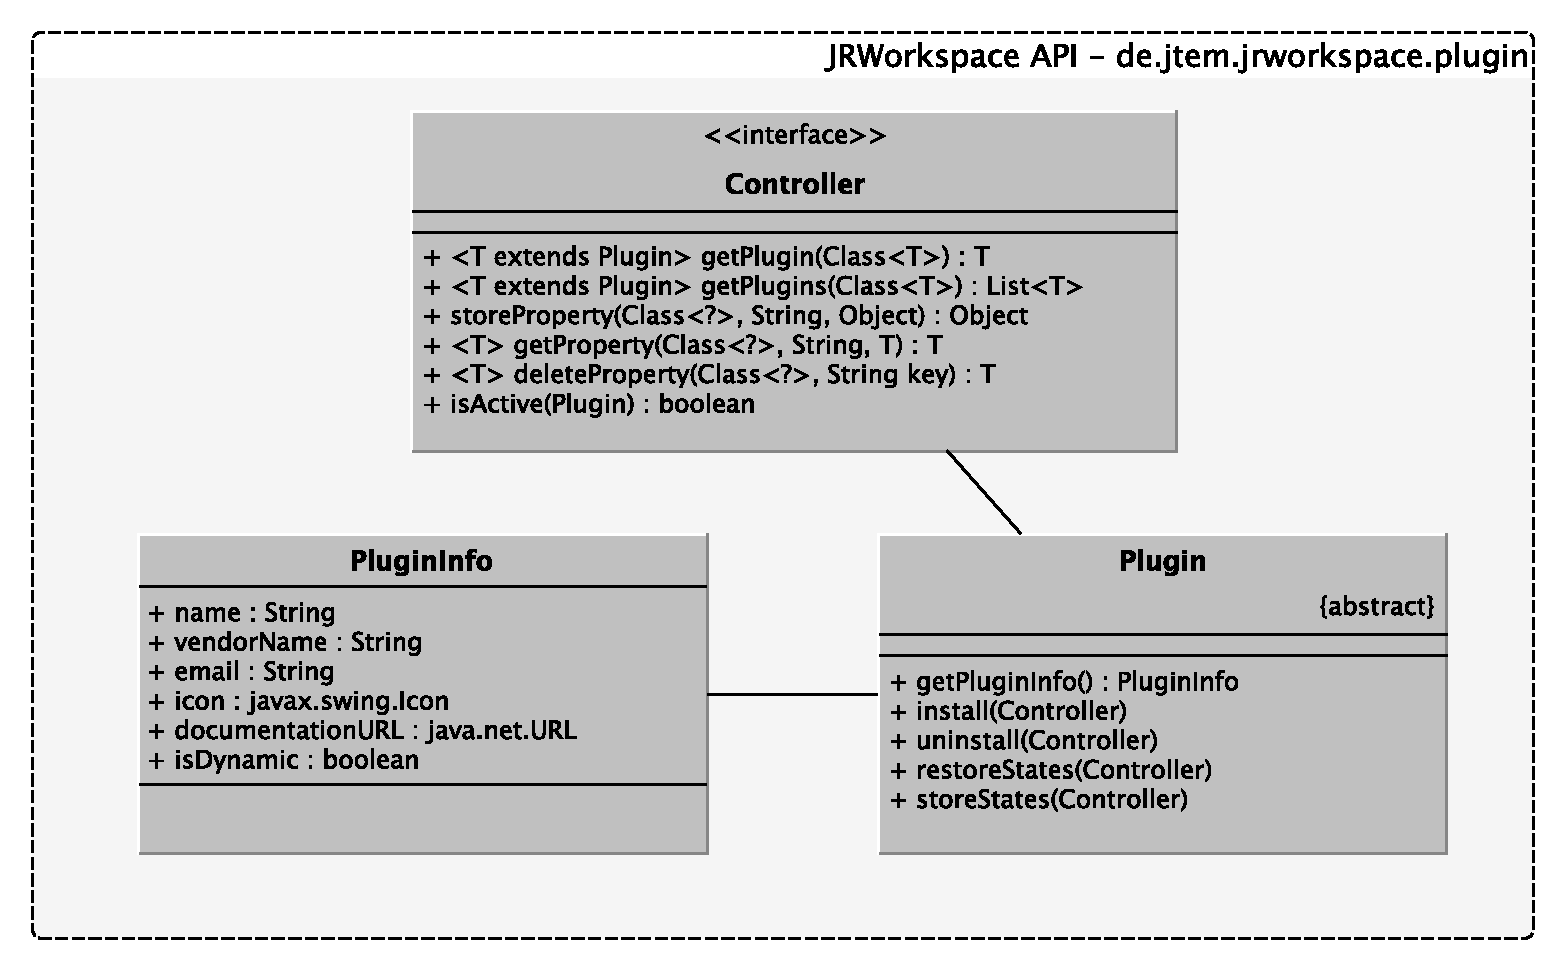
\includegraphics[width=0.8\linewidth]{figures/jrworkspace_uml}
%	\caption[{\sc JRworkspace} API]{
%		UML diagram for the {\sc JRworkspace} API.
%	}
%	\label{fig:jrworkspace_uml}
%\end{figure}

{\sc JRworkspace} is part of the {\sc Jtem} family of software projects 
\cite{JtemWebsite}. It defines a simple API to create modular Java applications. This API consists of
three basic classes (Listings~\ref{lst:plugin_base}, \ref{lst:controller_interface}, and 
\ref{lst:plugin_info}).
The project contains a reference implementation that supports the creation of Java
Swing applications using the {\sc JRworkspace} API. This implementation is used in all 
applications described in this work.

\subsection{Plug-ins and the controller}

In a {\sc JRworkspace} application a feature is implemented as plug-in and the corresponding Java class 
extends the abstract class Plugin
(Listing~\ref{lst:plugin_base}). The idea is that a plug-in can be installed by the controller 
calling its {\tt install} method or uninstalled via the {\tt uninstall} method. You can think of it 
as a feature added to your program. In particular there is no more than one instance of a
plug-in class in a {\sc JRworkspace} application.

A plug-in has a life-cycle during the runtime of the program which includes these basic
steps:
\begin{center}
\begin{tabular}{r|r|l}
	instantiation & 1 & set default plug-in state\\
	{\tt restoreStates} & 2 & load plug-in state from {\tt Controller}\\
	{\tt install} & 3 & calls {\tt getPlugin} to obtain dependent plug-ins\\
	{\tt --}  & 4 & program execution\\
	{\tt storeStates} & 5 & stores state values to the {\tt Controller}\\
	({\tt uninstall} & 6 & clean up)
\end{tabular}
\end{center}
Step 1 instantiates a plugin and initializes its default properties. In step 2 the controller 
calles the {\tt restoreStates} method. Step 3 is the actual installation of the plug-in. 
During runtime
of the application the plug-in can interact with possible user interface it created during 
installation or offer services to other plug-ins. 
Before program termination or before uninstall the {\tt storeStates} method is called. The plug-in
is supposed to store its state values by calling the {\tt storeProperty}
method of the controller.
Inter-plug-in-communication is done via the {\tt getPlugin} method of the controller. 
A plug-in should call {\tt getPlugin} from within the {\tt install} method to obtain the unique instance 
of a dependent plug-in. The {\tt getPlugin} method always returns the same instance of a plug-in so its
result can be stored by the {\tt install} method for later reference, see for example 
Listing~\ref{lst:sample_plugin}. Step 6 {\tt uninstall} is only used with dynamic plug-ins that support 
this operation. An implementation of {\tt Controller} may not support uninstallation of plug-ins.

We describe the basic API usage from a programmers point of view by giving an example plug-in
in Listing~\ref{lst:sample_plugin} and the source code of the three basic API classes 
{\tt Plugin}, {\tt Controller}, and {\tt PluginInfo} in Listings~\ref{lst:plugin_base}, 
\ref{lst:controller_interface}, and \ref{lst:plugin_info}.

\lstinputlisting[
	caption={
A simple plug-in class. It depends on a plug-in called {\tt DependentPlugin} 
and has the property {\tt doubleState}. It provides the method {\tt helloPlugin()} that 
prints some message. In the {\tt storeStates} method the value of {\tt doubleState} is
written to the controller. The class {\tt MyPlugin} is used as context class. The name of 
this class is used as name space to avoid property name ambiguities. The value of {\tt doubleState}
is read from the controller in the {\tt restoreStates} method using the same context class and
property name as in {\tt storeStates}. If there is no value with the given context and name
the default value {\tt 1.0} is returned by the {\tt getProperty} method. 
	},
	label=lst:sample_plugin,
	captionpos=b,
	firstline=6
] {java/de/sechel/thesis/MyPlugin.java}

\lstinputlisting[
	caption={
The {\tt Plugin} base class (excerpt). Note that plug-ins are equal if their classes are. 
It is not supported to have multiple instances of the same plug-in class installed.
	},
	label=lst:plugin_base,
	captionpos=b,
	firstline=3,
	lastline=30
] {java/de/jtem/jrworkspace/plugin/Plugin.java}

\lstinputlisting[
	caption={
The {\tt Controller} interface. A plug-in can obtain other plug-in instances by calling 
{\tt getPlugin} which returns a unique instance of the given plug-in class. The semantics
of the {\tt getPlugins} methods is different. It returns all plug-ins that are already known 
to the controller so no new dependencies are created by calling {\tt getPlugins}. Property
handling is done via the {\tt xxProperty} methods. Note that any {\tt Object} can be used
as property value. This requires the controller to use generic serialization to store data. It is 
strongly discouraged to use other classes than official java API classes as stored values as 
deserialization may fail if class geometry changes. 
	},
	label=lst:controller_interface,
	captionpos=b,
	firstline=5
] {java/de/jtem/jrworkspace/plugin/Controller.java}

\lstinputlisting[
	caption={
The plug-in meta data class (excerpt). Instances are returned by the {\tt getPluginInfo}
method of any plug-in. The value of the {\tt name} field is a plaintext name that could be 
shown in a user interface as well are the {\tt vendorName} and {\tt email} information. An optional 
{\tt icon} and a {\tt documentationURL} can be given. The flag {\tt isDynamic} isevaluated
by controller implementations that support deinstallation of plug-ins. A dynamic plug-in can
be installed or uninstalled during application runtime. A non-dynamic plug-in must be installed
at startup and remains installed until program termination. The static {\tt create} method returns
a default {\tt PluginInfo} instance for the given plug-in class.
	},
	label=lst:plugin_info,
	captionpos=b,
	firstline=7,
%	lastline=15
] {java/de/jtem/jrworkspace/plugin/PluginInfo.java}

In the next section we describe an implementation of this API.

\subsection{Reference implementation - {\tt SimpleController}}
This section describes a reference implementation of the {\sc JRworkspace} plug-in API.
It was started as a user interface framework for {\sc Jreality}~\cite{JrealityWebsite}. It implements
the {\tt Controller} interface in a class called {\tt SimpleController}. This name is historic
and did not change as the features evolved from simple into quite complex.
{\tt SimpleController} implements a {\sc Java Swing\TReg} framework for the creation of complex
modular applications based on the {\sc JRworkspace} API. It defines various plug-in flavors
that define user interface features.



\subsection{Gui elements}
\subsection{{\sc JRworkspace} and {\sc Jreality}}
\subsection{Building a {\sc JRworkspace} application}

\section{The {\sc Jtem} libraries {\sc Halfedge} and {\sc HalfedgeTools}}
\label{sec:halfedge_halfedgetools}
\subsection{The halfedge data structure and tools}
\subsection{Data model and algorithms}

\section{{\sc ConformalLab} - Conformal maps and uniformization}
\label{sec:conformallab}
\subsection{Embedded surfaces}
\subsection{Elliptic and hyperelliptic surfaces}
\subsection{Schottky data}
\subsection{Surfaces with boundary}

\section{{\sc VaryLab} - Variational methods for discrete surfaces}
\label{sec:varylab}
\subsection{Functional plug-ins}
\subsection{Implemented functionals and options}
\subsection{Remeshing}

\section{Non-linear optimization with {\sc Jpetsc/Jtao}}
\label{sec:jpetsctao}
\subsection{A java wrapper for {\sc PETSc/Tao}}

\section{{\sc U3D} - 3D content in presentations and online publiciations}
\label{sec:u3d}
\subsection{The {\sc Jreality} U3D export module}
\subsection{Discrete S-isothermic minimal surfaces}


%%% Local Variables:
%%% TeX-master: "Thesis.tex"
%%% End: